
%In addition, the \fitter references and GNU public licence are provided 
%together with the main source code. 
\fitter is an open source code licensed under the GNU general public licence. It can be downloaded from a dedicated 
webpage \cite{herafitter:page}
together with its supporting documentation and 
\emph{fast grid} theory files (described in section \ref{sec:techniques}) associated with data files.
The source code contains all the relevant information to perform QCD fits with HERA DIS data as a default 
set. \footnote{Default settings in \fitter are tuned to reproduce the central HERAPDF1.0 set.} 
The execution time depends on the fitting options and varies from 10 minutes 
(using ``FAST'' techniques as described in section \ref{sec:techniques}) to several hours when 
full uncertainties are estimated. The \fitter code is a combination of \tt C++ \rm and \tt Fortran 77\rm \ libraries with minimal 
dependencies, i.e. for the default fitting options no external dependencies are required except the \qcdnum evolution program \cite{qcdnum}.
% and CERN libraries. 
The \tt ROOT \rm  libraries are only required for the drawing tools and when invoking \applgrid.  
Drawing tools built into \fitter provide a qualitative and quantitative assessment of the results.
Fig.~\ref{fig:data} shows an illustration of a comparison between the inclusive NC data from HERA I
with the predictions based on HERAPDF1.0 PDFs.
The consistency of the measurements and the theory can be expressed by pulls, defined as the difference between data and theory divided by the uncorrelated error of the data. 
In each kinematic bin of the measurement, pulls are provided in units of standard deviations.  
The pulls are also illustrated in Fig.~\ref{fig:data}.
\begin{figure}[!ht]
   \centering
   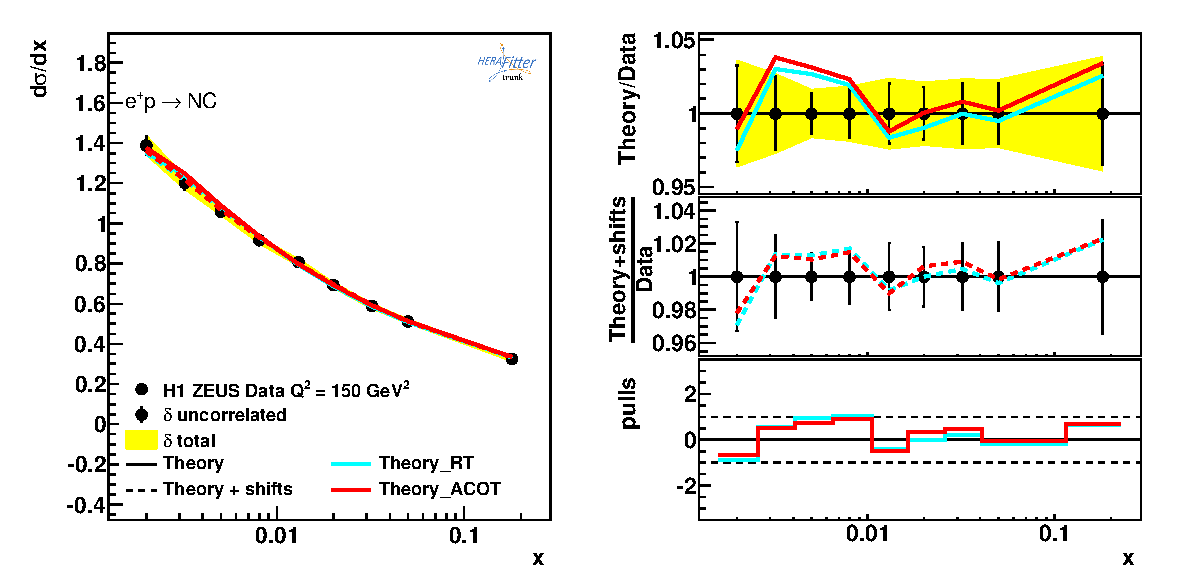
\includegraphics[width=8.6cm]{datatheory.pdf}
   \caption{An illustration of the consistency of HERA measurements~\cite{h1zeus:2009wt} and the theory predictions, 
       obtained in \fitter with the default drawing tool.} 
       %In addition, ratio plots are also provided together with the pull distribution (right panel).}    
 \label{fig:data}
\end{figure}


In \fitter there are also available cache options for fast retrieval, fast evolution kernels, and the OpenMP (Open Multi-Processing) 
interface which allows parallel applications of the GM-VFNS theory predictions in DIS. 


